\section{High Energy}
\subsection{Questions}
\begin{enumerate}
\item \textbf{Describe the mechanisms by which cosmic rays gain and lose energy. Which mechanisms
      are appropriate to which type of particle? Which ones produce electromagnetic
      radiation that we can observe, and in what wave bands?}
\item \textbf{Discuss the equation of state of relativistic/nonrelativistic degenerate gases of electrons
      and neutrons and derive the Chandrasekhar mass limit for white dwarfs. (A
      heuristic approach, as in Shapiro and Teukolsky, is sufficient.)}
\item \textbf{Derive the equation for the effective temperature of an accretion disk around a
      black hole of mass $M$ with accretion rate $\dot M$, as a function of radius $r$. Specify the
      assumptions required to get an answer, and comment on what could go wrong with
      them. Define the Eddington luminosity and explain its relevance to the peak frequency
      of the emitted radiation.}
\end{enumerate}

\subsection{Bondi Accrection}

Bondi accrection, also called spherical accretion, assumes your central object of mass $M$ is accreting isotropically from an ambient medium at infinity with density $\rho_\infty$, temperature $T_\infty$, $v_\infty = 0$, and sound speed $c_{s\infty}^2$. We're looking for a steady state solution, so $\nabla \cdot (\rho \underline{v}) = 0$ and $\frac{1}{2} v^2 + \phi + h = {\rm constant}$, which is Bernoulli's constant. Here, $\phi = \frac{-G M}{r}$, so we're neglecting self-gravity of the accreting fluid. We also have
\begin{equation}
h = \epsilon + \frac{P}{\rho} = \frac{1}{\Gamma - 1}\frac{P}{\rho} + \frac{P}{\rho} = \frac{c_s^2}{\Gamma - 1}\,\, ,
\end{equation}
where $\Gamma = 5/3$ for monatomic gas. Let's define the Bondi radius, which separates regimes where gravity is and is not dominant:
\begin{equation}
r_B = \frac{G M}{c_{s \infty}^2} \,\,.
\end{equation}
Now let's use Bernoulli's equation to relate the quantities when the gas is at infinity to the quantities at some radius $r$:
\begin{equation}
\frac{1}{2} v_r^2 - \frac{G M}{r} + \frac{1}{\Gamma - 1} c_s^2(r) = \frac{1}{\Gamma - 1} c_{s \infty}^2
\end{equation}
since at infinity, both $v_r$ and $\phi$ go to zero. Dividing out $c_{s \infty}^2$, this equation can be rewritten as 
\begin{equation}
\frac{1}{2}\frac{v_r^2(r)}{c_s^2(r)}\frac{c_s^2(r)}{c_{s \infty}^2(r)} - \frac{r_B}{r} + \frac{1}{\Gamma - 1}\frac{c_s^2(r)}{c_{s \infty}^2(r)} = \frac{1}{\Gamma - 1}
\end{equation}
Let's define here the Mach number $\mathcal{M} = \frac{v_r^2(r)}{c_s^2(r)}$. Also write $\rho_* = \frac{\rho}{\rho_\infty}$, and this equation becomes
\begin{equation}
\frac{\Gamma - 1}{2}\mathcal{M}^2 \rho_*^{\Gamma - 1} + \rho_*^{\Gamma - 1} = 1 + \frac{\Gamma - 1}{r_*}\,\, ,
\end{equation}
where $r_* = r/r_B$. We can use the fact that $4 \pi r^2 \rho v_r = \dot{M}$ is a constant with radius to eventually solve for the Mach number as a function of radius. There are lines of solutions, which matter will follow (some are not physical), shown in Figure \ref{f:mach}. The solutions that cross the sonic point ($\mathcal{M} = 1$) represent physical accretion and wind solutions. The descending curve is for accretion, and the ascending curve is for a wind that goes supersonic.

\begin{figure}[!h]
\begin{center}
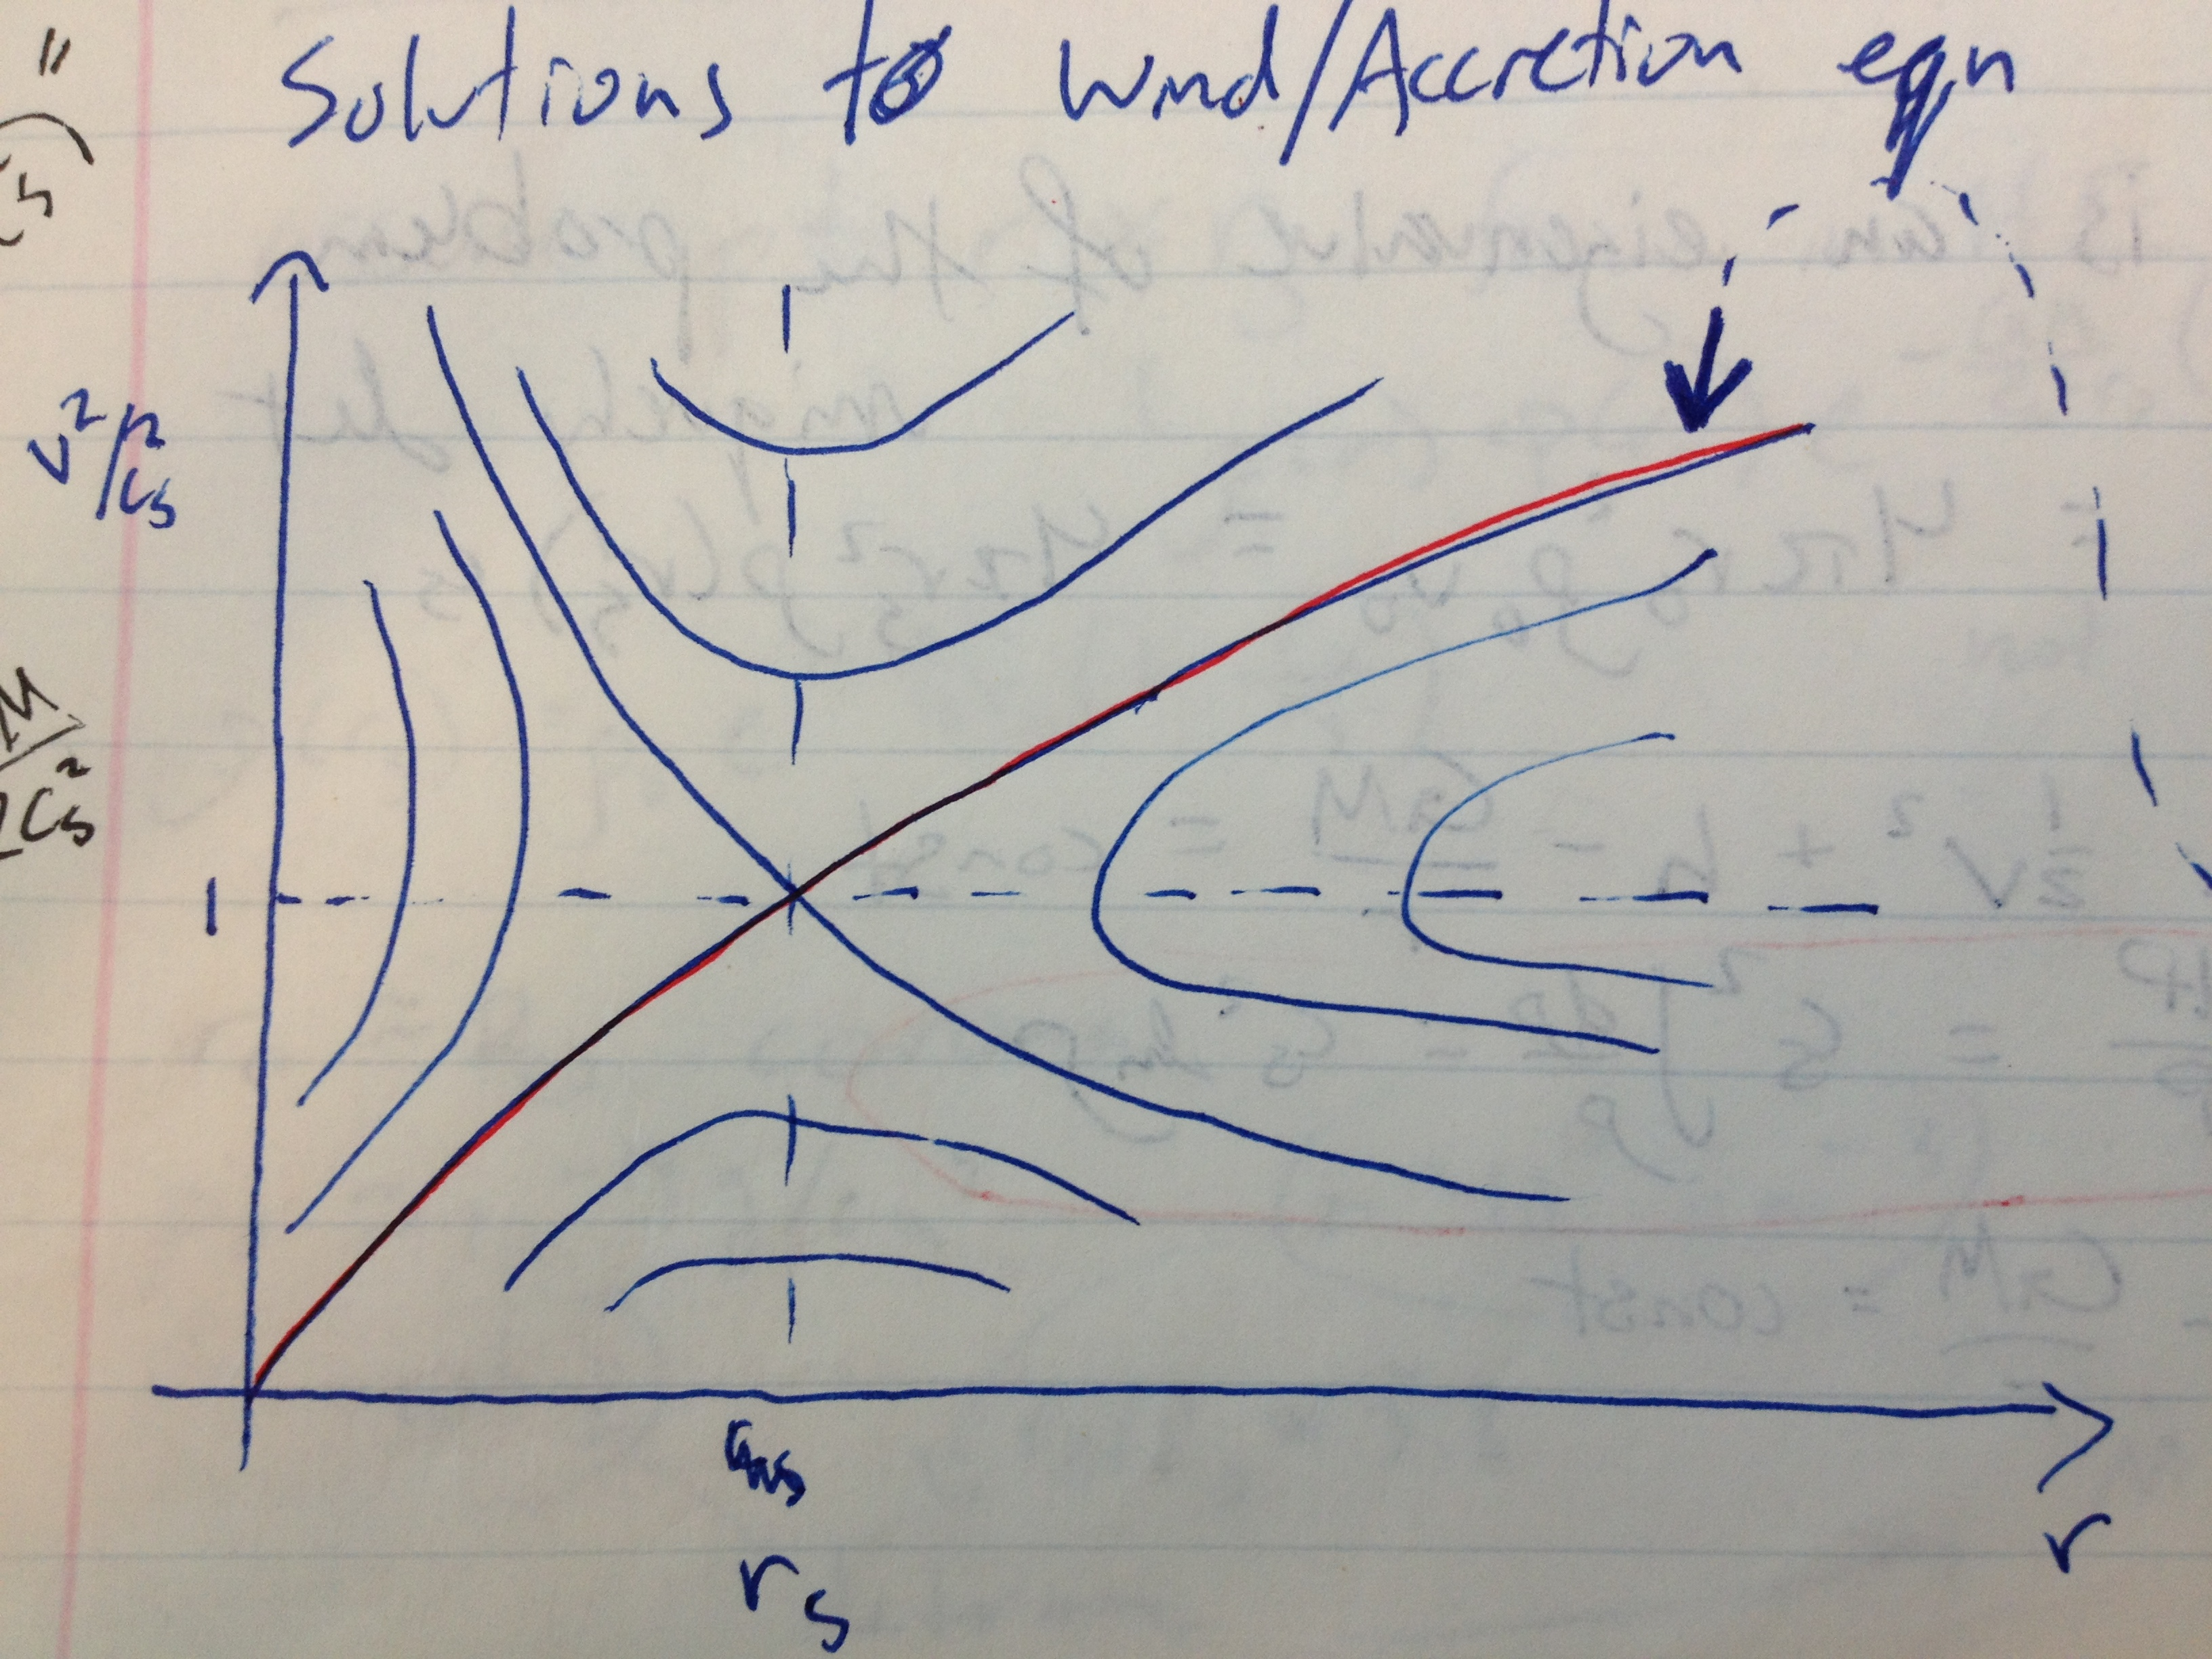
\includegraphics[width=\textwidth]{mach.jpg}
\caption{Mach number as a function of radius showing wind and accretion solutions \label{f:mach}}
\end{center}
\end{figure}

The sonic transition can be used to uniquely define $\dot{M}$:
\begin{equation}
\dot{M} = \lambda 4 \pi \biggl( \frac{G M}{c_{s \infty}^2} \biggr) ^2 \rho_\infty c_{s \infty}\,\, ,
\end{equation}
where $\lambda$ depends on $\Gamma$ and is $0.25$ for $\Gamma = 5/3$, $0.71$ for $\Gamma = 4/3$, $1.12$ for $\Gamma = 1$.

Let's also look at Bondi-Hoyle accretion, which is similar to Bondi accretion, except it's for a mass that's moving through the stuff it's accreting. This time, we can approximate:
\begin{equation}
\dot{M} = \pi \biggl(\frac{2 G M}{v_\infty ^2 + c_{s \infty}^2} \biggr)^2 \rho_* \sqrt{v_\infty ^2 + c_{s \infty}^2}\,\, .
\end{equation}
In this case, the incoming gas (from the perspective of the accreting mass) travels around the object and meets on the other side. This creates a shock in the gas, which heats and expands, and eventually this creates a bow shock around the accreting object as it moves through the fluid.



